The purpose of this analysis is to verify
that \texttt{\getsoftwarename{}} is able to reproduce the correct
power spectral density when using stochastically generated wind speed
time histories. These time histories are generated using a discrete
frequency function and Fast Fourier Transform, as described in
Wittig \& Sinha (1975) \cite{wittig1975simulation}. The calculated
power spectral density matrix for the generated time histories is compared to
an analytical spectral density matrix based on the Kaimal wind spectrum
model \cite{kaimal1972spectral, simiu1996wind} and the Davenport coherence
function \cite{davenport1967dependence}:

\begin{equation}
\bm{S}_{rs} = \sqrt{\bm{S}_{rr}(f) \cdot \bm{S}_{ss}(f)} Coh(f)
\end{equation}

\noindent where $\bm{S}_{rr}$ and $\bm{S}_{ss}$ are power spectral densities
of fluctuating wind at locations $r$ and $s$ respectively; $Coh(f)$ is the
Davenport coherence function; and $f$ is the frequency in Hz. This gives
the two-dimensional, $n$-variate power spectral density matrix $\bm{S}(f)$:

\begin{equation}
   \bm{S}(f) =
      \begin{bmatrix}
         S_{11}(f) & S_{12}(f) & \dots & S_{1n}(f) \\
         S_{21}(f) & S_{12}(f) & \dots & S_{2n}(f) \\
         \vdots & \vdots & \ddots & \vdots \\
         S_{n1}(f) & S_{n2}(f) & \dots & S_{nn}(f) \\         
      \end{bmatrix}
\end{equation}\\

\noindent The power spectral density based on the Kaimal wind spectrum is
defined as:

\begin{equation}
\bm{S}_{rr}(z_{r}, f) = u_{*}^{2} \cdot \frac{200 z_{r}}{\bar{U}(z_{r})} \cdot
              \frac{1}{\left[1 + 50 \frac{f z_{r}}{\bar{U}(z_{r})}\right]^{\frac{5}{3}}}
\end{equation}

\noindent where $\bm{S}_{rr}(f)$ is the power spectral density of the fluctuating
wind at location $z_{r}$ and frequency $f$ in Hz; $\bar{U}(z_{r})$ is
the mean wind speed at location $z_{r}$; and $u_{*}$ is the friction
velocity. The one-sided Davenport coherence function describes the correlation
between fluctuating winds at locations $z_{r}$ and $z_{s}$:

\begin{equation}
Coh(f) = \text{exp}\left[-\frac{C_{z}f\lvert z_{r} -
       z_{s}\rvert}{\frac{1}{2}\left[\bar{U}(z_{r}) + \bar{U}(z_{s})\right]}\right]
\end{equation}\\

\noindent The mean wind velocity at location $z_{r}$ is defined based on exposure conditions
defined in the ASCE 7 standard as follows:

\begin{equation}
\bar{U}(z) = \bar{b} \left(\frac{z}{33}\right)^{\bar{\alpha}}\left(\frac{88}{60}\right)V
\end{equation}

\noindent where $\bar{b}$ and $\bar{\alpha}$ are constants defined in ASCE 7 for
different exposure conditions; $V$ is the 3-second gust wind speed in miles
per hour.

\begin{figure}[!htbp]
  \centering {
    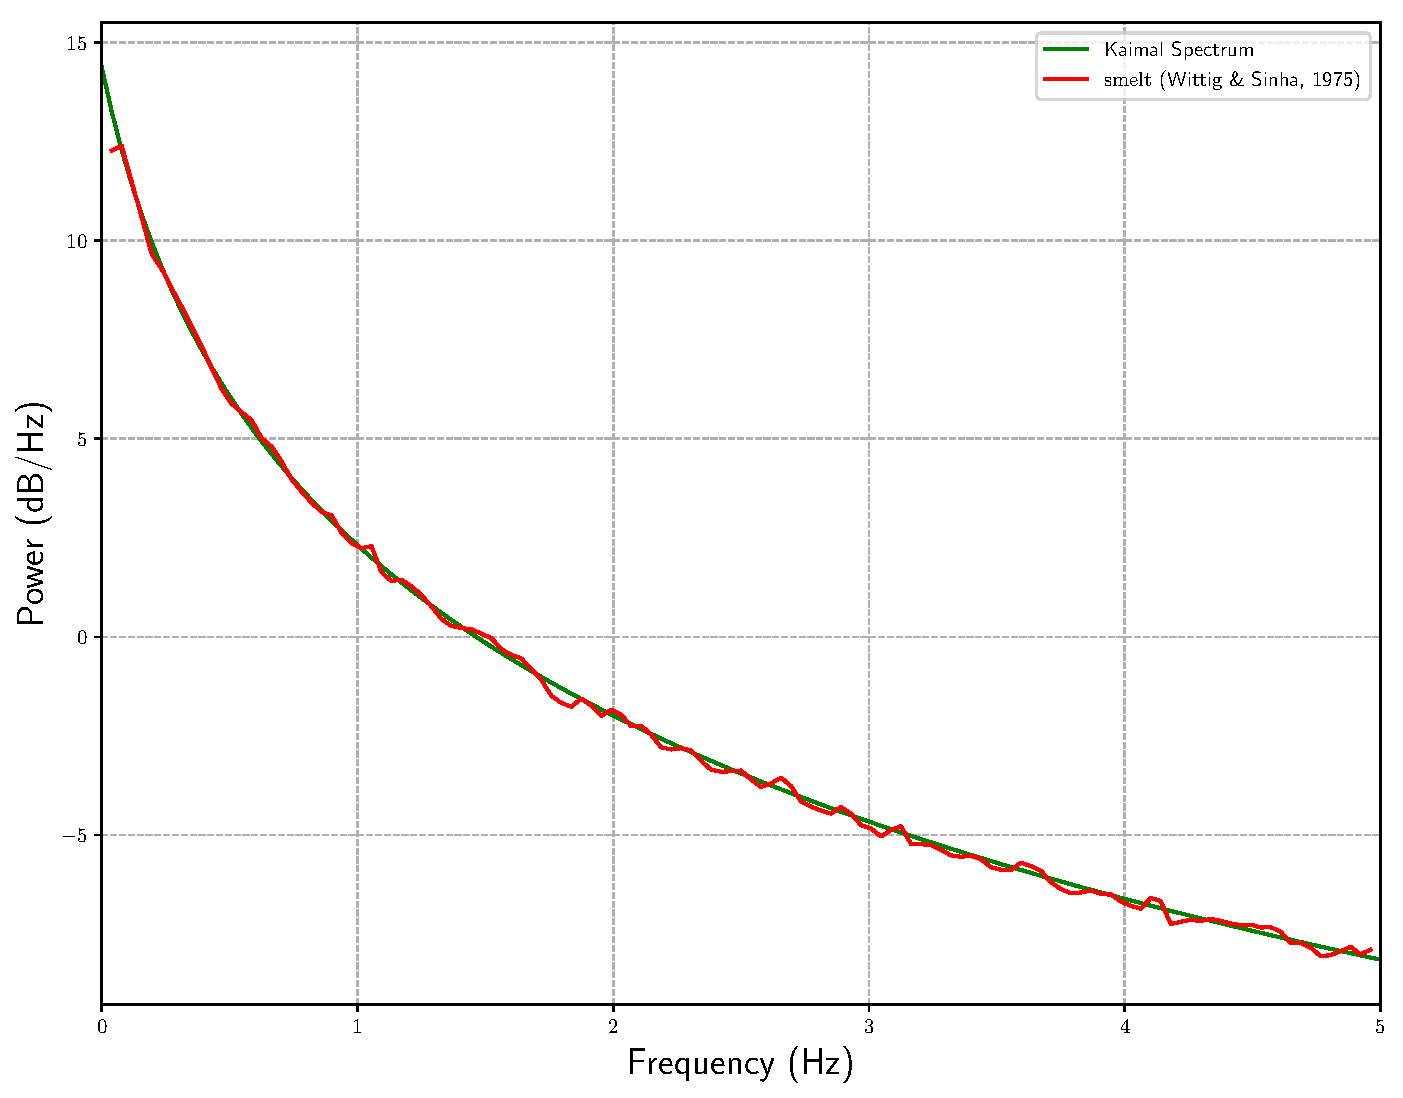
\includegraphics[width=0.8\textwidth]
    {./ver_and_val/figures/S11.pdf} }
  \caption{Comparison between theoretical and simulated auto power
    spectral density at the height of the first floor}
  \label{fig:auto_corr}
\end{figure}

\begin{figure}[!htbp]
  \centering {
    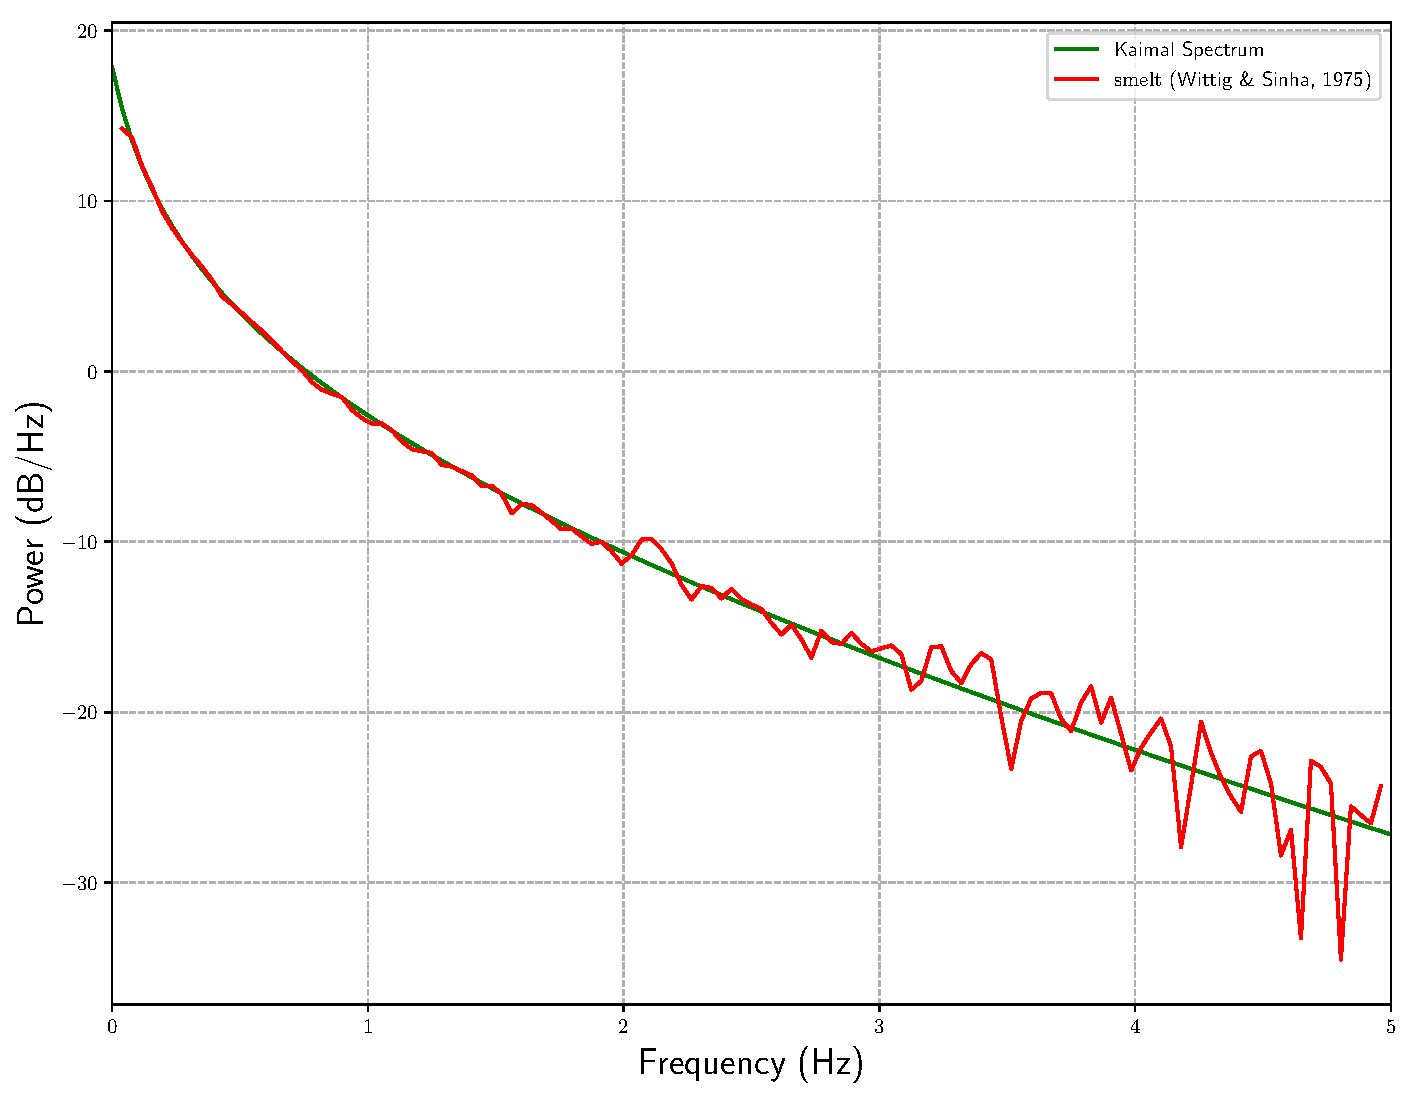
\includegraphics[width=0.8\textwidth]
    {./ver_and_val/figures/S23.pdf} }
  \caption{Comparison between theoretical and simulated cross power
    spectral density between the heights of the second and third floors}
  \label{fig:cross_corr}
\end{figure}

In the validation example, a 3-story structure with exposure category
D is subjected to wind loading with 3-second gust of 30 mph. An
estimate of the power spectral density matrix for the stochastic wind
velocity time history based on this condition was compared to the
power spectral density matrix calculated based on the Kaimal spectrum
with Davenport coherence. \Cref{fig:auto_corr} shows the auto correlation
for the first floor ($S_{11}$) while \Cref{fig:cross_corr} shows the cross
correlation between the second and third floors ($S_{23}$). As can be seen in
these two figures, the two different results show very good agreement
between the theoretical Kaimal values and the estimates based on the
generated stochastic wind velocity time histories. Further information
on the implementation of the Wittig \& Sinha (1975) model can be found
in the documentation
for \href{https://github.com/NHERI-SimCenter/smelt}{\texttt{smelt}}\textemdash
a C++ library for stochastically generating time histories for
different types of natural hazards.
